\chapter{Background} % enter the name of the chapter here

\section{AI}
Artificial Intelligence (AI) refers to the development of computer systems that can perform tasks that typically require human intelligence. These tasks include learning from experience, understanding natural language, recognizing patterns, solving problems, and making decisions. AI systems can be categorized into two main types: narrow or weak AI, which is designed for a specific task, and general or strong AI, which possesses human-like cognitive abilities across a range of tasks.
\section{machine-learning}
Machine Learning (ML) is a subfield of artificial intelligence (AI) that focuses on the development of algorithms and statistical models that enable computer systems to perform tasks without being explicitly programmed. The essence of machine learning lies in the ability of machines to learn from data, recognize patterns, and make decisions or predictions based on that learning.
\section{Neural Network}
A neural network is a computational model inspired by the structure and functioning of the human brain. It is a fundamental component of deep learning, a subset of machine learning. Neural networks consist of interconnected nodes, or artificial neurons, organized into layers. The three main types of layers in a neural network are the input layer, hidden layers, and output layer.
\subsection{Nodes}
In a neural network, nodes, also known as neurons or units, are fundamental building blocks that process and transmit information. Nodes are organized into layers, and each layer serves a specific function in the network. The three main types of layers in a neural network are the input layer, hidden layers, and output layer.
\begin{itemize}
    \item Input Layer:
        The input layer is the initial layer that receives raw data or features.
        Each node in the input layer represents a feature or attribute of the input data.
        The number of nodes in the input layer is determined by the dimensionality of the input data.
    \item Hidden Layers:
        Hidden layers are intermediate layers between the input and output layers.
        Each node in a hidden layer processes information and contributes to the network's ability to learn complex patterns.
        The term "hidden" arises because these layers are not directly observable in the input or output data.
    \item Output Layer:
        The output layer produces the final results or predictions of the neural network.
        The number of nodes in the output layer depends on the nature of the task. For example, in a binary \cite{chowdhury2020improving}classification task, there might be one node for each class, while in a regression task, there might be a single node.
\end{itemize}



Each connection between nodes is associated with a weight, which represents the strength of the connection. During training, these weights are adjusted to enable the network to learn from the input data and make accurate predictions.
\subsection{Activation Function}
An activation function is a crucial component in artificial neural networks and deep learning models. It introduces non-linearity to the network, allowing it to learn complex relationships in the data. The activation function operates on the input received by a node (or neuron) and produces an output that is used as the input for the next layer of the network.

Here are some commonly used activation functions in neural networks:
\begin{itemize}
    \item Sigmoid Function (Logistic Activation):\\
        Formula: 
\begin{equation}
        f(x) = \frac{1}{1 + e^{-x}}
\end{equation}
        Range: $(0, 1)$\\
        Used in the output layer of binary classification models to squash the output into a probability range.
    \item 
        Hyperbolic Tangent Function (tanh):\\
        Formula: 
        \begin{equation}
        f(x) = \frac{e^{2x} - 1}{e^{2x} + 1}
        \end{equation}
        Range: (-1, 1)\\
        Similar to the sigmoid function but with a broader output range. It is often used in hidden layers.
    \item 
        Rectified Linear Unit (ReLU):\\
        Formula: 
        \begin{equation}
            f(x) = \max(0, x)
        \end{equation}
        Range: $[0,\infty)[0,\infty)$\\
        Widely used in hidden layers due to its simplicity and effectiveness in training deep networks. However, it can suffer from the "dying ReLU" problem when neurons become inactive during training.
    \item 
        Leaky ReLU:\\
        Formula: 
        \begin{equation}
            f(x) = \max(\alpha x, x)
            \label{eq:}
        \end{equation}
        Introduces a small slope for negative values, addressing the dying ReLU problem.

\item        Parametric ReLU (PReLU):\\
        Similar to Leaky ReLU but allows the slope to be learned during training rather than being a fixed parameter.

    \item Exponential Linear Unit (ELU):\\
        Formula:
\begin{equation}
\text{ELU}(x) =
\begin{cases}
    x & \text{if } x \geq 0 \\
    \alpha(e^x - 1) & \text{if } x < 0
\end{cases}
\end{equation}
       A smooth alternative to ReLU that includes a saturation region for negative values.

\item         Softmax Function:\\
        Formula: 
\begin{equation}
\text{softmax}(x)_i = \frac{e^{x_i}}{\sum_j e^{x_j}}
\end{equation}
        Converts a vector of real numbers into a probability distribution. Often used in the output layer for multi-class classification problems.
\end{itemize}






\section{Deep-learning}
Deep learning is a subset of machine learning that involves the use of neural networks with multiple layers (deep neural networks) to model and solve complex problems. The term "deep" refers to the depth of the neural network, which is characterized by having multiple layers, often referred to as hidden layers, between the input and output layers.

\section{Natural Language Processing}
\cite{Rus2013}
Natural Language Processing (NLP) is a field of artificial intelligence (AI) that focuses on the interaction between computers and human languages. The goal of NLP is to enable machines to understand, interpret, and generate human-like text. This interdisciplinary field involves aspects of computer science, linguistics, and cognitive psychology.

\section{Language-Model}
A language model is a type of artificial intelligence (AI) model designed to understand and generate human-like text based on the input it receives. These models are trained on vast amounts of textual data and can be used for a variety of natural language processing (NLP) tasks.


\section{Large-Language-Model}
A large language model typically refers to a sophisticated artificial intelligence (AI) model designed for natural language processing (NLP) tasks and capable of handling vast amounts of textual data. These models have a high number of parameters, allowing them to capture intricate patterns and relationships in language. The size of a language model is often measured in terms of the number of parameters, which can range from millions to billions.


\section{Transformers in Deep Learning}
Transformers are a crucial architectural innovation in deep learning that revolutionized  natural language processing and other sequential data tasks. Introduced in the paper \cite{Attention} "Attention is All You Need" by Vaswani et al., transformers have become the foundation for various state-of-the-art models.



\subsection*{Key Components}
\begin{enumerate}
    \item \textbf{Self-Attention Mechanism:} Allows the model to focus on different parts of the input sequence while processing each element.
    \item \textbf{Multi-Head Attention:} Multiple self-attention heads run in parallel, capturing diverse aspects of relationships within the sequence.
    \item \textbf{Positional Encoding:} Incorporates information about the position of tokens in the input sequence, as transformers do not inherently understand the sequential order of data.
    \item \textbf{Feedforward Networks:} Non-linear transformations applied to the outputs of the attention mechanism.
\end{enumerate}

\subsection*{Advantages}
\begin{enumerate}
    \item \textbf{Parallelization:} Transformers enable parallel processing of input sequences, making them computationally efficient.
    \item \textbf{Capturing Long-Range Dependencies:} Self-attention allows transformers to capture relationships between distant elements in a sequence.
    \item \textbf{Versatility:} Initially designed for natural language processing, transformers have proven adaptable to various tasks, including image recognition and machine translation.
\end{enumerate}

\subsection*{Applications}
\begin{enumerate}
    \item \textbf{BERT (Bidirectional Encoder Representations from Transformers):} Introduced bidirectional context understanding for natural language understanding tasks.
    \item \textbf{GPT (Generative Pre-trained Transformer):} Utilizes transformers for autoregressive language modeling, generating coherent and contextually relevant text.
    \item \textbf{Image Transformers:} Applied to computer vision tasks, demonstrating competitive performance in image classification.
\end{enumerate}

\subsection*{Limitations}
\begin{enumerate}
    \item \textbf{Computational Complexity:} Transformers may be computationally expensive, particularly for large models.
    \item \textbf{Sequential Structure Understanding:} While transformers excel at parallel processing, they lack inherent understanding of sequential order.
\end{enumerate}

\section{BERT Model}
\cite{Bert}
BERT stands for Bidirectional Encoder Representations from Transformers and is a language representation model by Google.
This pre-trained model can be fine-tuned for a variety of final tasks that might not be similar to the task model was trained on.
BERT makes use of Transformer, an attention mechanism that learns contextual relations between words (or sub-words) in a text. In its vanilla form, Transformer includes two separate mechanisms — an encoder that reads the text input and a decoder that produces a prediction for the task. Since BERT’s goal is to generate a language model, only the encoder mechanism is necessary.
Historically, language models could only read text input sequentially -- either left-to-right or right-to-left -- but couldn't do both at the same time. BERT is different because it is designed to read in both directions at once. This capability, enabled by the introduction of Transformers, is known as bidirectionality.


\subsection{Model architecture}
L = Number of layers (i.e., \#Transformer encoder blocks in the stack).\\
H = Hidden size (i.e. the size of q, k and v vectors).\\
A = Number of attention heads.\\
BERT Base: L=12, H=768, A=12.\\
Total Parameters=110M!\\
BERT Large: L=24, H=1024, A=16.\\
Total Parameters=340M!!


\subsection{Pre-training BERT}
The BERT model is trained on the following two unsupervised tasks.
\begin{itemize}
    \item Masked Language Model (MLM)\\
        This task enables the deep bidirectional learning aspect of the model. In this task, some percentage of the input tokens are masked (Replaced with [MASK] token) at random and the model tries to predict these masked tokens — not the entire input sequence. The predicted tokens from the model are then fed into an output softmax over the vocabulary to get the final output words.
    \item  Next Sentence Prediction (NSP)\\
        It is a technique used in BERT to help the model understand the relationship between two consecutive sentences. In simple terms, NSP is designed to teach BERT how sentences are connected and whether they logically follow each other.
\end{itemize}





\section{Fine tuning} % enter the name of the section here
\cite{Fine-Tune}
Fine tuning is a machine-learning technique that involves making small changes to a pre-trained model to improve its performance on a specific task and helps the model better understand the specific context and language patterns of the task it is being fine-tuned for. This is more efficient and often yields better results than training a model from scratch, as the model already has a good understanding of the world and can use this knowledge to learn the new task more quickly. 
Suppose a healthcare organization wants to use LLM to assist doctors in generating patient reports from textual notes. While this model can understand and create general text, it might not be optimized for intricate medical terms and specific healthcare jargon, So to enhance its performance for this specialized role, the organization fine-tunes the model on a dataset filled with medical reports and patient notes.
And after fine-tuning, the model is primed to assist doctors in generating accurate and coherent patient reports, demonstrating its adaptability for specific tasks.
If we didn’t use this approach, we would initially have random weights. In that case, a complex architecture would require a lot of time for training.
So briefly, fine-tuning refers to using the weights of an already trained network as the starting values for training a new network.


\subsection{Why Fine-Tuning?} %enter the name of the subsection here

\begin{itemize}
    \item \textbf{Transfer Learning:} Pre-trained models have already learned useful features from large datasets. Fine-tuning allows us to use this knowledge and apply it to a new related task. It's like taking knowledge gained in one area and using it in another.
    
    \item \textbf{Efficiency:} Training a model from scratch can be computationally expensive and time-consuming. Fine-tuning is more efficient since it starts with a model that has already learned a lot and then refines it for a specific task.
    
    \item \textbf{Limited Data:} In many real-world scenarios, collecting large amounts of labelled data for training a model from scratch might be impractical. Fine-tuning helps when you have limited data because the pre-trained model already has a good understanding of the general features or language meanings.
    
    \item \textbf{Domain-Specific Tasks:} Models trained on general tasks can be fine-tuned for more specific tasks in a particular domain. For example, a model trained on general text can be fine-tuned for sentiment analysis in customer reviews.
\end{itemize}

\subsection{Capabilities of an LLM after Fine tuning}
\begin{figure}[h]
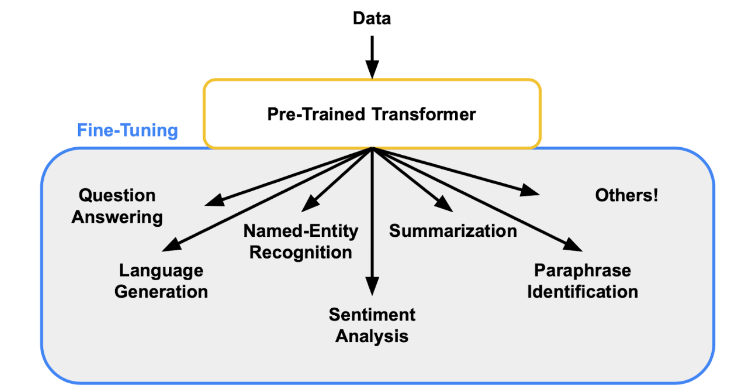
\includegraphics[scale=0.8]{finetune}\\
\centering
\end{figure}
\begin{itemize}
    \item Sentiment Analysis: Boost the model performance in understanding and categorizing emotions and opinions in textual content.
    \item Named Entity Recognition (NER): For tasks that involve pinpointing the names of individuals, organizations, locations, and various entities, fine-tuning the model can significantly enhance its precision and accuracy in recognizing and classifying these key elements.
    \item Text Generation: Fine-tuning is a powerful tool for customizing the model's text generation abilities. This process allows you to make the model's output to follow to specific writing styles, tones, or themes.
    \item Question Answering: When dealing with tasks that require answering questions based on contextual information we may using fine tuning. It equips the model with the ability to understand and extract relevant details, enabling it to provide accurate and context-aware responses.
\end{itemize}


\subsection{Supervised fine-tuning:}
Supervised fine-tuning is a process in machine learning which we are using a pre-trained model, and trying to adapted it for a specific task using labelled data. In this approach, the model's parameters are adjusted based on a clear set of input-output pairs, where the output is known and provided during the training phase. The objective is for the model to learn the intricate patterns and relationships within the labelled data, allowing it to generalize its understanding to new, similar examples and enhancing its performance in making accurate predictions or classifications.


\subsubsection {The approach involves the following steps:}
\begin{enumerate}
    \item Choose the fine-tuning task, such as text generation or analysis.
    \item Prepare datasets containing questions and answers related to the chosen topic. Specify prompts for generating questions and completing tasks.
    \item Select the base model, e.g., "arabert."
    \item Fine-tune the model using a supervised approach, specifying relevant parameters and training methods.
    \item Evaluate the performance of the fine-tuned model using appropriate metrics.
\end{enumerate}



\subsection {Reinforcement Learning Overview}
\cite{cruz2023reinforcement}
Reinforcement Learning (RL) is a machine learning training method that rewards desired behaviors and penalizes undesired ones. It involves an agent perceiving and interpreting its environment, taking actions, and learning through trial and error. Key components include the agent, environment, observation, state, action, reward, and policy.
\subsection*{How Reinforcement Learning Works}
RL involves an agent exploring an unknown environment to achieve a goal, maximizing expected cumulative reward. The main elements include the agent, environment, policy, and reward signal. The value function captures the 'goodness' of a state, and the Bellman equation is a key concept in RL, used for calculating value functions.

\subsection*{Approaches to Implement RL Algorithms}
Three approaches:

\begin{figure}[h]
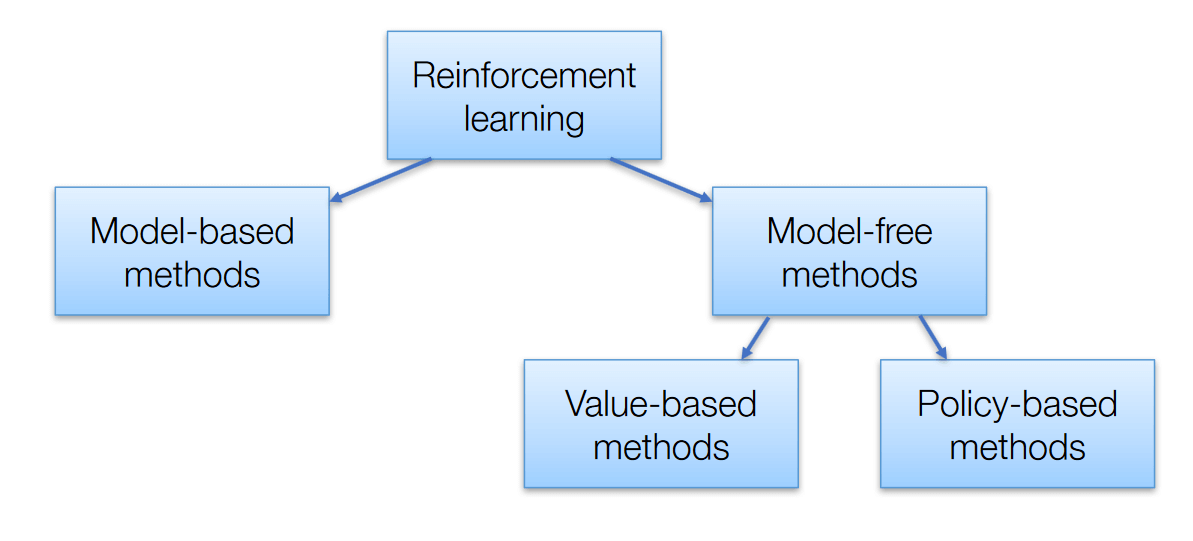
\includegraphics[scale=0.3]{rml}\\
\centering
\end{figure}
\begin{enumerate}
    \item \textbf{Value-Based:} Maximizing a value function.
    \item \textbf{Policy-Based:} Developing a strategy for maximum future rewards.
    \item \textbf{Model-Based:} Creating a virtual model to assist learning in a specific environment.
\end{enumerate}

\subsection*{Bellman Equation}
Utilizes the action, state, reward, discount factor, and value of the starting point to estimate values and maximize rewards.
The key-elements used in Bellman equations are:
\begin{itemize}
    \item Action performed by the agent is referred to as "a"
    \item State occurred by performing the action is "s."
    \item The reward/feedback obtained for each good and bad action is "R."
    \item A discount factor is Gamma "$\gamma$."
    \item The value of your starting point is the reward you expect to get from being there, plus the value of wherever you land next.
    \item {On-Policy Value Functions}
        The Bellman equation for the on-policy value functions is given by:
        \begin{equation}
            V^{\pi}(s) = \sum_a \pi(a|s) \sum_{s', r} p(s', r|s, a) \left[r + \gamma V^{\pi}(s')\right]
        \end{equation}
    \item The corresponding update rule for the action-value function is:
        \begin{equation}
            Q^{\pi}(s, a) = \sum_{s', r} p(s', r|s, a) \left[r + \gamma \sum_{a'} \pi(a'|s') Q^{\pi}(s', a')\right]
        \end{equation}

    \item {Optimal Value Functions}

        The Bellman equation for the optimal value functions is given by:
        \begin{equation}
            V^*(s) = \max_a \sum_{s', r} p(s', r|s, a) \left[r + \gamma V^*(s')\right]
        \end{equation}
    \item The corresponding update rule for the optimal action-value function is:
        \begin{equation}
            Q^*(s, a) = \sum_{s', r} p(s', r|s, a) \left[r + \gamma \max_{a'} Q^*(s', a')\right]
        \end{equation}
\end{itemize}



\subsection*{Q-Learning}
\begin{figure}[h]
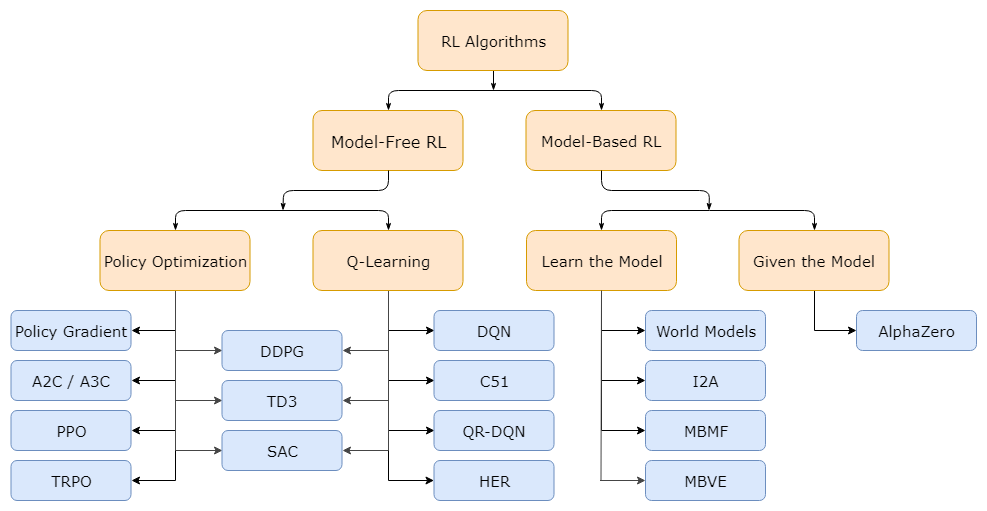
\includegraphics[scale=0.4]{optiq}\\
\centering
\end{figure}
A common RL algorithm that approximates the optimal action-value function. Q-learning methods learn an approximator for the optimal action-value function, typically using an objective function based on the Bellman equation.
\begin{equation}
Q(s, a) = \sum_{s', r} p(s', r \mid s, a) \left[ r + \gamma \max_{a'} Q(s', a') \right]
\end{equation}
\subsection*{Types of Reinforcement Learning}

\begin{figure}
\centering
\begin{tikzpicture}[>=stealth, node distance=2.5cm, every node/.style={rectangle, draw, align=center}]

% Nodes
\node (positive) {Positive Reinforcement \\ Strengthens behavior by \\ rewarding with positive stimuli};
\node (negative) [below=0.5cm of positive] {Negative Reinforcement \\ Strengthens behavior by \\ removing or avoiding negative stimuli};
\node (punishment) [below=0.5cm of negative] {Punishment \\ Weakens behavior by applying \\ negative stimuli};
\node (extinction) [below=0.5cm of punishment] {Extinction \\ Weakens behavior by removing \\ reinforcement, leading to behavior fade};

% Arrows
\draw[->] (positive) -- (negative);
\draw[->] (negative) -- (punishment);
\draw[->] (punishment) -- (extinction);

\end{tikzpicture}
\caption{Types of Reinforcement Learning}
\end{figure}
\begin{enumerate}
    \item \textbf{Positive Reinforcement:} Strengthens and increases behavior.
    \item \textbf{Negative Reinforcement:} Strengthens behavior by avoiding negative conditions.
\end{enumerate}

\subsection*{Reinforcement Learning Applications}
\begin{itemize}
    \item \textbf{Robotics:} Navigation, Robo-soccer, etc.
    \item \textbf{Control:} Adaptive control in factory processes, telecommunication, etc.
    \item \textbf{Game Playing:} Tic-tac-toe, chess, etc.
    \item \textbf{Chemistry:} Optimizing chemical reactions.
    \item \textbf{Business:} Strategy planning.
    \item \textbf{Manufacturing:} Robotic tasks in various industries.
    \item \textbf{Finance Sector:} Evaluating trading strategies.
\end{itemize}


\subsection{What is wanas?}
Wanas is conceptualized as a therapist that acts as a supportive friend to help individuals navigate daily mental challenges. The approach involves designing a model where different sub-models handle specific therapeutic tasks, and a larger model decides which sub-model to deploy at different times. The design process drew inspiration from interviews with therapists to understand how they communicate with patients, aiming to create interactions that bring happiness and a positive outlook to individuals' lives. This approach seeks to emulate the empathetic and uplifting qualities of human therapeutic interactions in an AI-driven model.


\subsubsection{How therapist function?}
\begin{itemize}
    \item \textbf{Active Listening:} Therapists practice active listening, fully concentrating, understanding, responding, and remembering what the client is saying.
    \item \textbf{Empathy:} Showing empathy involves understanding and sharing the feelings of the client, expressing genuine understanding through verbal and non-verbal cues.
    \item \textbf{Open-ended Questions:} Therapists ask open-ended questions to encourage clients to share more about their thoughts and feelings.
    \item \textbf{Reflective Responses:} Therapists use reflective responses, paraphrasing or summarizing what the client has said to demonstrate active listening.
    \item \textbf{Clarification:} Seeking clarification when there is ambiguity or when more information is needed to ensure a shared understanding.
    \item \textbf{Non-verbal Communication:} Paying attention to non-verbal cues such as body language, facial expressions, and tone of voice.
    \item \textbf{Validation:} Validating the client's experiences and emotions without judgment to build a trusting relationship.
    \item \textbf{Encouragement:} Offering encouragement to motivate clients to explore difficult topics and recognize their strengths and progress.
    \item \textbf{Cultural Sensitivity:} Being mindful of cultural differences and adapting communication styles to be sensitive to the client's cultural background.
    \item \textbf{Respect and Non-judgment:} Communicating with respect and without judgment to create a safe space for clients to share openly.
    \item \textbf{Feedback:} Providing constructive feedback in a supportive and collaborative manner to help clients gain insights into their behavior and thought patterns.
    \item \textbf{Goal Setting:} Collaboratively setting therapeutic goals to ensure focused and aligned therapy that empowers clients to take an active role in their own growth.
    \item \textbf{Boundaries:} Communicating and maintaining clear professional boundaries to ensure a safe and ethical therapeutic relationship.


    \item \textbf{Trauma-Informed Communication:} Using trauma-informed communication for clients who have experienced trauma, prioritizing safety and avoiding retraumatization.
\end{itemize}
\subsection{AraBert}
\cite{Arabert}
Arabic BERT," is a pre-trained language model designed specifically for the Arabic language. BERT, or Bidirectional Encoder Representations from Transformers, is a transformer-based model developed by Google that has proven to be highly effective in capturing context and semantics in natural language.

AraBERT, as an adaptation of BERT for Arabic, has been trained on a large corpus of Arabic text to understand the nuances and intricacies of the language. This pre-training allows AraBERT to generate high-quality contextualized embeddings for Arabic words and sentences. These embeddings can then be fine-tuned for specific downstream tasks, such as sentiment analysis, named entity recognition, or other natural language processing tasks in the Arabic language domain.

In summary, AraBERT is a powerful tool for natural language processing in Arabic, leveraging the strengths of BERT's architecture while specifically tailored for the characteristics of the Arabic language.
which is traied on many datasets such as 
\subsection{Our Goal}
The goal is to create multiple specialized models for distinct tasks,
allowing the system to choose the most appropriate model based on patient responses.
This involves fine-tuning a Language Model (LLM),
such as AraBert, which has been pre-trained on extensive Arabic datasets.
The pre-training equips the model with a comprehensive understanding of Arabic language rules,
enabling it to effectively handle various language-related tasks in a healthcare or therapeutic context.


